\documentclass[11pt]{article}
\usepackage[margin=1in]{geometry}
\usepackage{amsmath,amssymb}
\usepackage{booktabs}
\usepackage{graphicx}
\usepackage{microtype}
\usepackage[font=small,labelfont=bf]{caption}
\usepackage[hidelinks]{hyperref}
\usepackage{natbib}
\graphicspath{{../figures/}}
% written by paper/make_numbers.py from results/, do not edit by hand
\newcommand{\RawRows}{2{,}312{,}944}
\newcommand{\CleanApps}{2{,}241{,}891}
\newcommand{\CohortApps}{815{,}231}
\newcommand{\SimApps}{799{,}763}
\newcommand{\TrainApps}{334{,}566}
\newcommand{\TestApps}{480{,}665}
\newcommand{\AblTrainApps}{135{,}263}
\newcommand{\WindowApps}{1{,}959{,}938}
\newcommand{\Developers}{736{,}124}
\newcommand{\NeverUpdated}{21.6\%}
\newcommand{\OldReportedAUC}{0.862}
\newcommand{\OldReportedLogit}{0.840}
\newcommand{\AUCLaunch}{0.836}
\newcommand{\LoLaunch}{0.831}
\newcommand{\HiLaunch}{0.841}
\newcommand{\BrierLaunch}{0.0417}
\newcommand{\BSSLaunch}{0.122}
\newcommand{\SlopeLaunch}{0.92}
\newcommand{\IntLaunch}{$-$0.05}
\newcommand{\ECELaunch}{0.0036}
\newcommand{\TopTenLaunch}{47\%}
\newcommand{\DiffLaunch}{0.000}
\newcommand{\DiffLoLaunch}{0.000}
\newcommand{\DiffHiLaunch}{0.000}
\newcommand{\AUCLaunchLogit}{0.825}
\newcommand{\LoLaunchLogit}{0.820}
\newcommand{\HiLaunchLogit}{0.830}
\newcommand{\BrierLaunchLogit}{0.0425}
\newcommand{\BSSLaunchLogit}{0.106}
\newcommand{\SlopeLaunchLogit}{0.99}
\newcommand{\IntLaunchLogit}{$-$0.06}
\newcommand{\ECELaunchLogit}{0.0036}
\newcommand{\TopTenLaunchLogit}{45\%}
\newcommand{\DiffLaunchLogit}{$-$0.011}
\newcommand{\DiffLoLaunchLogit}{$-$0.013}
\newcommand{\DiffHiLaunchLogit}{$-$0.009}
\newcommand{\AUCStrict}{0.711}
\newcommand{\LoStrict}{0.704}
\newcommand{\HiStrict}{0.718}
\newcommand{\BrierStrict}{0.0454}
\newcommand{\BSSStrict}{0.044}
\newcommand{\SlopeStrict}{0.86}
\newcommand{\IntStrict}{0.01}
\newcommand{\ECEStrict}{0.0033}
\newcommand{\TopTenStrict}{31\%}
\newcommand{\DiffStrict}{$-$0.126}
\newcommand{\DiffLoStrict}{$-$0.131}
\newcommand{\DiffHiStrict}{$-$0.120}
\newcommand{\AUCBaseCatDev}{0.750}
\newcommand{\LoBaseCatDev}{0.743}
\newcommand{\HiBaseCatDev}{0.757}
\newcommand{\BrierBaseCatDev}{0.0448}
\newcommand{\BSSBaseCatDev}{0.056}
\newcommand{\SlopeBaseCatDev}{1.02}
\newcommand{\IntBaseCatDev}{0.01}
\newcommand{\ECEBaseCatDev}{0.0024}
\newcommand{\TopTenBaseCatDev}{33\%}
\newcommand{\DiffBaseCatDev}{$-$0.086}
\newcommand{\DiffLoBaseCatDev}{$-$0.090}
\newcommand{\DiffHiBaseCatDev}{$-$0.082}
\newcommand{\AUCBaseCat}{0.726}
\newcommand{\LoBaseCat}{0.719}
\newcommand{\HiBaseCat}{0.733}
\newcommand{\BrierBaseCat}{0.0453}
\newcommand{\BSSBaseCat}{0.047}
\newcommand{\SlopeBaseCat}{0.97}
\newcommand{\IntBaseCat}{$-$0.00}
\newcommand{\ECEBaseCat}{0.0037}
\newcommand{\TopTenBaseCat}{31\%}
\newcommand{\DiffBaseCat}{$-$0.110}
\newcommand{\DiffLoBaseCat}{$-$0.116}
\newcommand{\DiffHiBaseCat}{$-$0.104}
\newcommand{\AUCBaseDev}{0.593}
\newcommand{\LoBaseDev}{0.585}
\newcommand{\HiBaseDev}{0.602}
\newcommand{\BrierBaseDev}{0.0472}
\newcommand{\BSSBaseDev}{0.006}
\newcommand{\SlopeBaseDev}{1.19}
\newcommand{\IntBaseDev}{$-$0.01}
\newcommand{\ECEBaseDev}{0.0022}
\newcommand{\TopTenBaseDev}{13\%}
\newcommand{\DiffBaseDev}{$-$0.243}
\newcommand{\DiffLoBaseDev}{$-$0.250}
\newcommand{\DiffHiBaseDev}{$-$0.235}
\newcommand{\AUCOld}{0.861}
\newcommand{\LoOld}{0.857}
\newcommand{\HiOld}{0.865}
\newcommand{\BrierOld}{0.0395}
\newcommand{\BSSOld}{0.169}
\newcommand{\SlopeOld}{0.90}
\newcommand{\IntOld}{$-$0.11}
\newcommand{\ECEOld}{0.0052}
\newcommand{\TopTenOld}{53\%}
\newcommand{\DiffOld}{0.025}
\newcommand{\DiffLoOld}{0.021}
\newcommand{\DiffHiOld}{0.029}
\newcommand{\AUCOldLogit}{0.845}
\newcommand{\LoOldLogit}{0.839}
\newcommand{\HiOldLogit}{0.849}
\newcommand{\BrierOldLogit}{0.0405}
\newcommand{\BSSOldLogit}{0.147}
\newcommand{\SlopeOldLogit}{1.00}
\newcommand{\IntOldLogit}{$-$0.07}
\newcommand{\ECEOldLogit}{0.0029}
\newcommand{\TopTenOldLogit}{50\%}
\newcommand{\DiffOldLogit}{0.008}
\newcommand{\DiffLoOldLogit}{0.004}
\newcommand{\DiffHiOldLogit}{0.012}
\newcommand{\AUCOldHundredK}{0.861}
\newcommand{\WithinOldHundredK}{0.861}
\newcommand{\AUCLaunchHundredK}{0.835}
\newcommand{\WithinLaunchHundredK}{0.834}
\newcommand{\SimPopApps}{472{,}059}
\newcommand{\SimPopLaunch}{0.834}
\newcommand{\SimPopOld}{0.859}
\newcommand{\AblOld}{0.857}
\newcommand{\AblOldNoMon}{0.816}
\newcommand{\AblOldNoMonList}{0.801}
\newcommand{\AblOldNoSnap}{0.748}
\newcommand{\AblMonOnly}{0.746}
\newcommand{\AblLaunch}{0.830}
\newcommand{\AblLaunchMon}{0.858}
\newcommand{\AblLaunchSnap}{0.876}
\newcommand{\AblLaunchLeakyDev}{0.893}
\newcommand{\AblLaunchPost}{0.984}
\newcommand{\AblNoTitle}{0.783}
\newcommand{\AblNoCategory}{0.779}
\newcommand{\SnapShare}{30\%}
\newcommand{\GapShare}{8\%}
\newcommand{\SeedLaunchMean}{0.831}
\newcommand{\SeedLaunchSD}{0.0009}
\newcommand{\SeedOldMean}{0.859}
\newcommand{\SeedOldSD}{0.0007}
\newcommand{\ShiftLaunchA}{0.824}
\newcommand{\ShiftOldA}{0.864}
\newcommand{\ShiftLaunchB}{0.825}
\newcommand{\ShiftOldB}{0.854}
\newcommand{\ShiftLaunchC}{0.813}
\newcommand{\ShiftOldC}{0.824}
\newcommand{\SensOneLaunch}{0.874}
\newcommand{\SensOneOld}{0.911}
\newcommand{\SensTenLaunch}{0.788}
\newcommand{\SensTenOld}{0.817}
\newcommand{\RecallOverall}{47\%}
\newcommand{\PrecisionTop}{23.5\%}
\newcommand{\Link}{cloglog}
\newcommand{\FTenKTwelve}{13.6\%}
\newcommand{\FTenKTwelveLo}{13.1\%}
\newcommand{\FTenKTwelveHi}{14.0\%}
\newcommand{\FTenKThirtySix}{21.6\%}
\newcommand{\FTenKThirtySixLo}{20.4\%}
\newcommand{\FTenKThirtySixHi}{22.3\%}
\newcommand{\FwdAUCTenK}{0.740}
\newcommand{\FwdWAUCTenK}{0.754}
\newcommand{\FwdLLTenK}{0.3498}
\newcommand{\FwdAgeLLTenK}{0.3937}
\newcommand{\IntAUCTenK}{0.761}
\newcommand{\IntWAUCTenK}{0.742}
\newcommand{\IntLLTenK}{0.4145}
\newcommand{\IntAgeLLTenK}{0.4694}
\newcommand{\FwdSlopeYearTenK}{1.17}
\newcommand{\FwdIntYearTenK}{0.35}
\newcommand{\FHundredKTwelve}{3.7\%}
\newcommand{\FHundredKTwelveLo}{3.5\%}
\newcommand{\FHundredKTwelveHi}{3.8\%}
\newcommand{\FHundredKThirtySix}{7.0\%}
\newcommand{\FHundredKThirtySixLo}{6.5\%}
\newcommand{\FHundredKThirtySixHi}{7.4\%}
\newcommand{\FwdAUCHundredK}{0.797}
\newcommand{\FwdWAUCHundredK}{0.808}
\newcommand{\FwdLLHundredK}{0.1354}
\newcommand{\FwdAgeLLHundredK}{0.1575}
\newcommand{\IntAUCHundredK}{0.811}
\newcommand{\IntWAUCHundredK}{0.794}
\newcommand{\IntLLHundredK}{0.1883}
\newcommand{\IntAgeLLHundredK}{0.2208}
\newcommand{\FwdSlopeYearHundredK}{1.10}
\newcommand{\FwdIntYearHundredK}{0.40}
\newcommand{\FOneMTwelve}{0.68\%}
\newcommand{\FOneMTwelveLo}{0.61\%}
\newcommand{\FOneMTwelveHi}{0.75\%}
\newcommand{\FOneMThirtySix}{1.69\%}
\newcommand{\FOneMThirtySixLo}{1.53\%}
\newcommand{\FOneMThirtySixHi}{1.82\%}
\newcommand{\FwdAUCOneM}{0.855}
\newcommand{\FwdWAUCOneM}{0.859}
\newcommand{\FwdLLOneM}{0.0362}
\newcommand{\FwdAgeLLOneM}{0.0432}
\newcommand{\IntAUCOneM}{0.867}
\newcommand{\IntWAUCOneM}{0.852}
\newcommand{\IntLLOneM}{0.0592}
\newcommand{\IntAgeLLOneM}{0.0721}
\newcommand{\FwdSlopeYearOneM}{0.98}
\newcommand{\FwdIntYearOneM}{0.27}
\newcommand{\LLCloglog}{0.1972}
\newcommand{\LLProbit}{0.1993}
\newcommand{\LLLogit}{0.1976}
\newcommand{\CovEighty}{80.1\%}
\newcommand{\CovNinety}{90.1\%}
\newcommand{\CovFifty}{50.1\%}
\newcommand{\CovEightyFwd}{80.7\%}
\newcommand{\WidthEighty}{0.73}
\newcommand{\CovGames}{75.2\%}
\newcommand{\WidthFifty}{0.44}
\newcommand{\WidthNinety}{0.84}
\newcommand{\WidthEightyFwd}{0.73}
\newcommand{\FitSample}{400{,}000}
\newcommand{\FwdMeanPredHundredK}{2.7\%}
\newcommand{\FwdRateHundredK}{3.6\%}
\newcommand{\IntSlopeHundredK}{0.98}
\newcommand{\SimFirstTenK}{44.0\%}
\newcommand{\BusFirstTenK}{4.5\%}
\newcommand{\TopTenCorr}{$-$0.24}
\newcommand{\RawApps}{102{,}979}
\newcommand{\RawTenK}{13.0\%}
\newcommand{\RawHundredK}{3.45\%}
\newcommand{\RawOneM}{0.64\%}
\newcommand{\RawModelHundredK}{3.6\%}
\newcommand{\RawFlatLo}{13.0\%}
\newcommand{\RawFlatHi}{14.1\%}
\newcommand{\RawObsEarly}{13.2\%}
\newcommand{\RawModelEarly}{10.4\%}
\newcommand{\RawObsLate}{14.4\%}
\newcommand{\RawModelLate}{16.6\%}
\newcommand{\SimObsApps}{717}
\newcommand{\SimObsTenK}{36.3\%}
\newcommand{\SimModelTenK}{43.0\%}
\newcommand{\BusObsApps}{7{,}628}
\newcommand{\BusObsTenK}{4.5\%}
\newcommand{\BusModelTenK}{4.5\%}
\newcommand{\CatInsideTenK}{46\%}
\newcommand{\CatInsideHundredK}{52\%}
\newcommand{\CatRatioMin}{0.71}
\newcommand{\CatRatioMax}{2.09}
\newcommand{\NpmleSimCoverage}{85\%}
\newcommand{\NpmleSimNominal}{95\%}
\newcommand{\NpmleSimApps}{200{,}000}
\newcommand{\RRAdsIapAll}{3.09}
\newcommand{\RRAdsIapAllLo}{2.95}
\newcommand{\RRAdsIapAllHi}{3.24}
\newcommand{\EAdsIapAll}{5.64}
\newcommand{\ECIAdsIapAll}{5.36}
\newcommand{\RRAdsIapNever}{1.97}
\newcommand{\RRAdsIapNeverLo}{1.55}
\newcommand{\RRAdsIapNeverHi}{2.52}
\newcommand{\EAdsIapNever}{3.36}
\newcommand{\ECIAdsIapNever}{2.46}
\newcommand{\RRAdsIapUpd}{2.83}
\newcommand{\RRAdsIapUpdLo}{2.71}
\newcommand{\RRAdsIapUpdHi}{2.96}
\newcommand{\EAdsIapUpd}{5.11}
\newcommand{\ECIAdsIapUpd}{4.86}
\newcommand{\RRIapOnlyAll}{1.67}
\newcommand{\RRIapOnlyAllLo}{1.57}
\newcommand{\RRIapOnlyAllHi}{1.77}
\newcommand{\EIapOnlyAll}{2.73}
\newcommand{\ECIIapOnlyAll}{2.52}
\newcommand{\RRIapOnlyNever}{1.25}
\newcommand{\RRIapOnlyNeverLo}{0.80}
\newcommand{\RRIapOnlyNeverHi}{1.96}
\newcommand{\EIapOnlyNever}{1.81}
\newcommand{\ECIIapOnlyNever}{1.00}
\newcommand{\RRIapOnlyUpd}{1.54}
\newcommand{\RRIapOnlyUpdLo}{1.45}
\newcommand{\RRIapOnlyUpdHi}{1.63}
\newcommand{\EIapOnlyUpd}{2.45}
\newcommand{\ECIIapOnlyUpd}{2.26}
\newcommand{\RRNoMonAll}{0.26}
\newcommand{\RRNoMonAllLo}{0.25}
\newcommand{\RRNoMonAllHi}{0.27}
\newcommand{\ENoMonAll}{7.22}
\newcommand{\ECINoMonAll}{6.87}
\newcommand{\RRNoMonNever}{0.24}
\newcommand{\RRNoMonNeverLo}{0.18}
\newcommand{\RRNoMonNeverHi}{0.32}
\newcommand{\ENoMonNever}{7.86}
\newcommand{\ECINoMonNever}{5.75}
\newcommand{\RRNoMonUpd}{0.26}
\newcommand{\RRNoMonUpdLo}{0.25}
\newcommand{\RRNoMonUpdHi}{0.27}
\newcommand{\ENoMonUpd}{7.15}
\newcommand{\ECINoMonUpd}{6.80}
\newcommand{\RRPaidAll}{0.20}
\newcommand{\RRPaidAllLo}{0.16}
\newcommand{\RRPaidAllHi}{0.24}
\newcommand{\EPaidAll}{9.54}
\newcommand{\ECIPaidAll}{7.67}
\newcommand{\RRPaidNever}{0.13}
\newcommand{\RRPaidNeverLo}{0.05}
\newcommand{\RRPaidNeverHi}{0.38}
\newcommand{\EPaidNever}{14.43}
\newcommand{\ECIPaidNever}{4.69}
\newcommand{\RRPaidUpd}{0.20}
\newcommand{\RRPaidUpdLo}{0.17}
\newcommand{\RRPaidUpdHi}{0.25}
\newcommand{\EPaidUpd}{9.26}
\newcommand{\ECIPaidUpd}{7.44}
\newcommand{\RRPrivacyAll}{3.64}
\newcommand{\RRPrivacyAllLo}{3.39}
\newcommand{\RRPrivacyAllHi}{3.90}
\newcommand{\EPrivacyAll}{6.73}
\newcommand{\ECIPrivacyAll}{6.24}
\newcommand{\RRPrivacyNever}{2.72}
\newcommand{\RRPrivacyNeverLo}{2.27}
\newcommand{\RRPrivacyNeverHi}{3.26}
\newcommand{\EPrivacyNever}{4.88}
\newcommand{\ECIPrivacyNever}{3.96}
\newcommand{\RRPrivacyUpd}{3.37}
\newcommand{\RRPrivacyUpdLo}{3.13}
\newcommand{\RRPrivacyUpdHi}{3.63}
\newcommand{\EPrivacyUpd}{6.20}
\newcommand{\ECIPrivacyUpd}{5.72}
\newcommand{\RRWebsiteAll}{1.86}
\newcommand{\RRWebsiteAllLo}{1.78}
\newcommand{\RRWebsiteAllHi}{1.93}
\newcommand{\EWebsiteAll}{3.12}
\newcommand{\ECIWebsiteAll}{2.96}
\newcommand{\RRWebsiteNever}{1.12}
\newcommand{\RRWebsiteNeverLo}{0.97}
\newcommand{\RRWebsiteNeverHi}{1.30}
\newcommand{\EWebsiteNever}{1.49}
\newcommand{\ECIWebsiteNever}{1.00}
\newcommand{\RRWebsiteUpd}{1.76}
\newcommand{\RRWebsiteUpdLo}{1.68}
\newcommand{\RRWebsiteUpdHi}{1.83}
\newcommand{\EWebsiteUpd}{2.91}
\newcommand{\ECIWebsiteUpd}{2.76}
\newcommand{\IapHitsUpd}{37\%}
\newcommand{\IapHitsNever}{12\%}
\newcommand{\IapHitsRatio}{3.14}
\newcommand{\NeverHits}{5\%}
\newcommand{\NeverRest}{22\%}


\title{What Can You Know on Launch Day?\\[2pt]
\large Leakage, Horizons and Calibration in Predicting Google Play Success}
\author{Matin Nikoomanzar\\ University of California, Los Angeles}
\date{October 2026}

\begin{document}
\maketitle

\begin{abstract}
\noindent I revisit a model that predicted which new Google Play apps reach 100K installs. It scored an AUC of
\OldReportedAUC{} on a 2018 to 2019 temporal split, but most of its inputs (monetization, size, privacy policy,
content rating) were read off a June 2021 snapshot, years after launch, and its outcome gave older apps more time to
grow. I build a feature availability table, keep only inputs that were known on launch day, and redefine success so
every app gets the same horizon. Ranking apps by whether they end up in the top 5\% of their launch month, the
launch-time model scores \AUCLaunch{} (95\% CI \LoLaunch{} to \HiLaunch{}) against \AUCOld{} for the old feature
set on the same split, with a calibration slope of \SlopeLaunch{}. For absolute horizons I treat the single snapshot
as current status survival data, estimate time to 10K, 100K and 1M installs with the NPMLE and a parametric
(\Link{}) model on launch covariates, and validate it forward in time. Pooled over launch cohorts, \FHundredKTwelve{}
of apps reach 100K installs within a year of launch, while the raw rate for apps 11 to 13 months old is
\RawHundredK{}, so the pooled curve hides some cohort drift. The model is well calibrated when held-out launch months
are interleaved with training months and under-predicts when it is fit on older launches only. I also give split
conformal intervals with checked coverage, which are wide, and I bound the monetization associations with E-values
instead of reading them as effects.
\end{abstract}

\section{Introduction}

App stores are a good place to study winner-take-most markets. On Google Play a tiny share of apps collect almost
all installs, so the practical question for a developer or an early investor is whether you can tell, on launch day,
which apps will be in that group. An earlier version of this project answered yes, with an AUC of \OldReportedAUC{}.
There are two problems with that answer. The inputs included things nobody could know on launch day, and the
outcome gave apps released in early 2018 more than twice as long to grow as apps released in late 2019.

This paper is the rebuild. The research question is narrow on purpose:

\begin{quote}
Using only information available on an app's launch day, how well can you rank and give calibrated probabilities for
its eventual success, measured on a horizon that is the same for every app?
\end{quote}

The question can fail. If launch-day facts carried no signal, the AUC would be near 0.5 and the honest conclusion
would be that the old model only worked because it peeked. That is not what happens. The gap between the two
numbers, and where it comes from, is the main result.

\section{Data}

The data is a scrape of \RawRows{} Google Play listings from June 15 and 16, 2021 \citep{prakash2021}. After dropping
rows with no release date, install count or category I keep \CleanApps{} apps from \Developers{} developers. Each app is seen exactly once.
Install counts (\texttt{Maximum Installs}) are cumulative and close to exact. Only apps still listed in June 2021 are
present, so failed apps are under-represented and more so for older launch years. I come back to this in Section~\ref{sec:limits}. \NeverUpdated{} of apps were never updated after their release date. The old analysis used the
\CohortApps{} apps released in 2018 and 2019. The live simulator was trained on \SimApps{} of them (those with a
known size and one of the four main content ratings), which is where the two app counts on the project website come
from.

\section{What was known on launch day}

Table~\ref{tab:avail} summarizes the availability table in \texttt{docs/method.md}. Every input any model uses is
tagged as known at launch, known only in the 2021 snapshot, or only defined after launch, together with a judgment of
whether success can change it. A test fails if anything not tagged ``launch'' enters a launch-time model. A second test shuffles each app's own
installs, ratings, monetization flags, size and update fields and checks that its launch features do not move. A third
changes the installs, in-app purchase flag and title of apps released after a cutoff and checks that no launch feature
of an earlier app moves. None of these tests can say whether a tagged ``launch'' field was edited later, which is why the
table has an ``editable'' row.

\begin{table}[h]
\centering\small
\begin{tabular}{lp{7.2cm}l}
\toprule
Group & Examples & First known \\
\midrule
Launch, fixed & release date, package name, developer's earlier releases & launch day \\
Launch, editable & category, app title (the title is the weaker case, since developers rewrite it for search) & launch day (2021 value used) \\
Snapshot & price, ads, in-app purchases, size, minimum Android, content rating, privacy policy, website & June 2021 \\
After launch & ratings, rating count, editors' choice, last update, earlier apps' installs & June 2021 \\
\bottomrule
\end{tabular}
\caption{Feature availability. The old model used eight snapshot fields plus category and developer app count.}
\label{tab:avail}
\end{table}

The developer app count in the old model was built correctly in time (it ranks a developer's apps by release date),
but it only counts apps that survived to 2021, and its labels in the write-up were off by one. A developer's
\emph{track record}, meaning how many earlier apps became hits, looks like launch information but is not, because those apps'
installs were also counted in 2021, after the launch being predicted.

\section{A consistent horizon}

\paragraph{Ranking target.} An app is a hit if its installs are in the top 5\% of all apps released in the same
calendar month. Every app is compared only with apps that had the same time to grow. The base rate is 5\% in every
month by construction.

\paragraph{Absolute target.} App $i$ is observed once, at age $a_i$, with $\delta_i = 1\{T_i \le a_i\}$, where
$T_i$ is the time to reach $N$ installs. This is current status data. Without covariates the NPMLE of
$F(t) = P(T \le t)$ is the isotonic regression of $\delta$ on $a$ \citep{groeneboom1992}. It converges at rate
$n^{1/3}$, and the plain bootstrap is known to fail for cube-root estimators of this kind \citep{sen2010}, so I
use subsampling with the cube-root rate \citep{politis1994}. With launch covariates $x$ I fit
\begin{equation}
P(T \le t \mid x) = G(\alpha + \beta \log t + x^\top\gamma),
\end{equation}
where $G$ is the complementary log-log (Weibull proportional hazards), probit (log-normal AFT) or logistic
(log-logistic AFT) link. Each implies a time ratio $\exp(-\gamma_j/\beta)$ for covariate $j$. The model assumes no
cohort effect, so given $x$ the time to milestone does not depend on launch date. One snapshot cannot test that in
sample, because age and launch date are the same thing, so I test it out of sample.

\section{Ranking results}

All ranking models train on 2018 launches (\TrainApps{} apps) and are scored on 2019 launches (\TestApps{} apps).
Confidence intervals come from 500 bootstrap draws that resample whole developers.

\begin{table}[h]
\centering\small
\begin{tabular}{lcccc}
\toprule
Model & AUC [95\% CI] & Brier & Cal.\ slope & Top 10\% finds \\
\midrule
Category rate & \AUCBaseCat{} [\LoBaseCat, \HiBaseCat] & \BrierBaseCat & \SlopeBaseCat & \TopTenBaseCat \\
Developer history rate & \AUCBaseDev{} [\LoBaseDev, \HiBaseDev] & \BrierBaseDev & \SlopeBaseDev & \TopTenBaseDev \\
Category $\times$ developer & \AUCBaseCatDev{} [\LoBaseCatDev, \HiBaseCatDev] & \BrierBaseCatDev & \SlopeBaseCatDev & \TopTenBaseCatDev \\
Launch, strict (no category or title) & \AUCStrict{} [\LoStrict, \HiStrict] & \BrierStrict & \SlopeStrict & \TopTenStrict \\
Launch, spline logistic & \AUCLaunchLogit{} [\LoLaunchLogit, \HiLaunchLogit] & \BrierLaunchLogit & \SlopeLaunchLogit & \TopTenLaunchLogit \\
\textbf{Launch, gradient boosting} & \textbf{\AUCLaunch{}} [\LoLaunch, \HiLaunch] & \BrierLaunch & \SlopeLaunch & \TopTenLaunch \\
\midrule
Old features, logistic & \AUCOldLogit{} [\LoOldLogit, \HiOldLogit] & \BrierOldLogit & \SlopeOldLogit & \TopTenOldLogit \\
Old features, gradient boosting & \AUCOld{} [\LoOld, \HiOld] & \BrierOld & \SlopeOld & \TopTenOld \\
\bottomrule
\end{tabular}
\caption{2019 launches, top 5\% of launch month. The old feature set uses 2021 snapshot fields and is shown for
comparison only. Paired difference old minus launch: \DiffOld{} [\DiffLoOld, \DiffHiOld].}
\label{tab:main}
\end{table}

\begin{figure}[!htb]
\centering
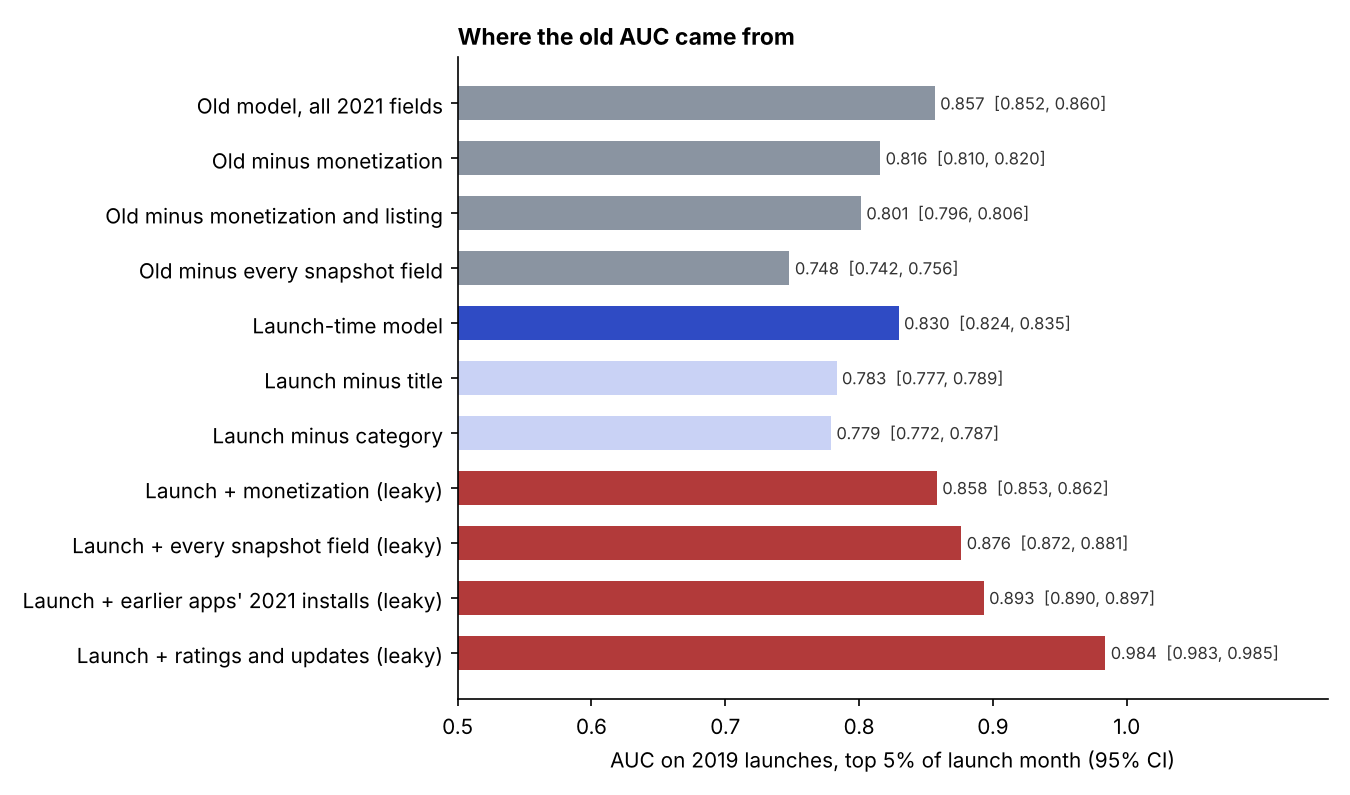
\includegraphics[width=0.7\linewidth]{7_leakage_ablation.png}
\caption{The leakage ablation on 2019 launches, all fit on the same \AblTrainApps{} training apps (a 40\% sample of
training developers).}
\label{fig:cal}
\end{figure}

\paragraph{Where the old AUC came from.} On the old outcome (100K by June 2021) the old feature set scores
\AUCOldHundredK{} in my refit, close to the \OldReportedAUC{} in the original report. Scored within launch month, which removes the free credit for being
older, it scores \WithinOldHundredK{}. On the horizon-consistent target the ablation in Figure~\ref{fig:cal} gives
\AblOld{} for the old features, \AblOldNoMon{} without monetization, \AblOldNoSnap{} with every snapshot field
removed, and \AblLaunch{} for the launch features. Dropping the title features from the launch set gives
\AblNoTitle{} and dropping category gives \AblNoCategory{}. The title is a 2021 value that developers edit, so part of
its signal may come from changes made after launch. Adding the three monetization flags back to the launch set gives
\AblLaunchMon{}, all snapshot fields \AblLaunchSnap{}, earlier apps' 2021 installs \AblLaunchLeakyDev{}, and the 2021
ratings and update fields \AblLaunchPost{}, which shows how fast a model can look brilliant when it is allowed to read
the outcome. Removing every snapshot field from the old features costs \SnapShare{} of the old model's lift over an
AUC of 0.5, but that comparison is against a weak model (category and developer app count only). Against the full
launch model the gap is \GapShare{} of that lift, because the launch set also has developer history features that
the old set lacked. Scoring within launch month leaves the old AUC unchanged (\WithinOldHundredK{} against
\AUCOldHundredK{}), so among 2019 launches the unequal horizon did not inflate the ranking number. That check covers
twelve launch months and cannot rule out inflation over the 2016 to 2020 range. The unequal horizon does change the
100K rate, which falls with launch year in the data.

\paragraph{Calibration and stability.} The launch model's calibration slope is \SlopeLaunch{} and its intercept
\IntLaunch{} (Figure~\ref{fig:rel}). Three refits on different halves of the training developers give AUC \SeedLaunchMean{} with standard
deviation \SeedLaunchSD{} (old features: \SeedOldMean{}, \SeedOldSD{}).

\begin{figure}[!htb]
\centering
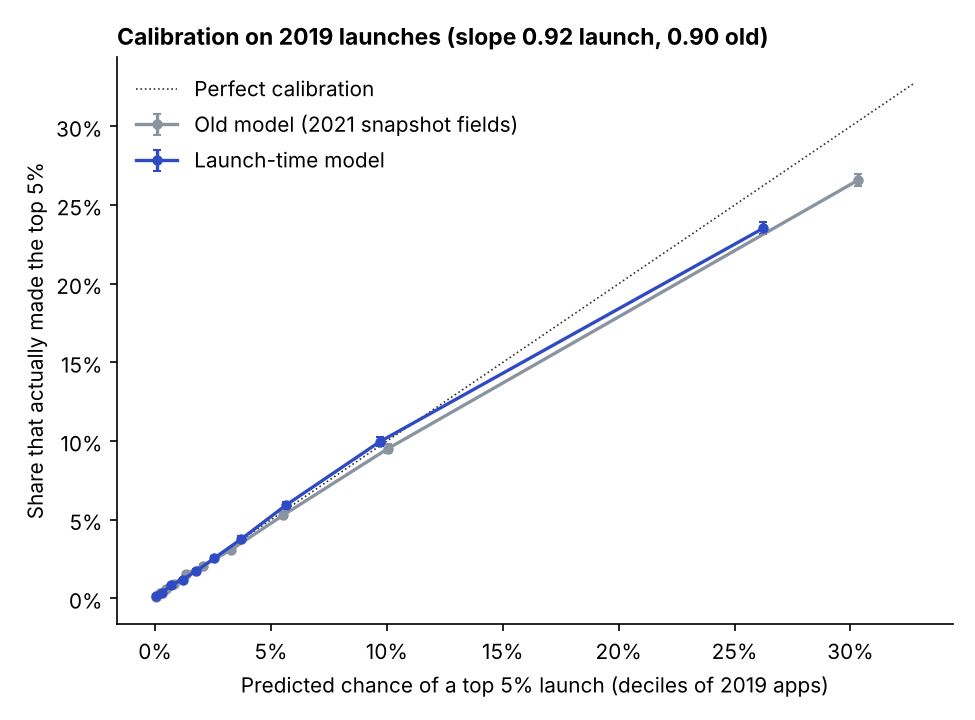
\includegraphics[width=0.5\linewidth]{6_calibration.png}
\caption{Reliability on 2019 launches by decile of predicted probability, with Wilson intervals.}
\label{fig:rel}
\end{figure}

\paragraph{Shift.} Trained on 2016 and 2017 launches, the launch model scores \ShiftLaunchA{}, \ShiftLaunchB{} and
\ShiftLaunchC{} on 2018, 2019 and 2020 launches (old features: \ShiftOldA{}, \ShiftOldB{}, \ShiftOldC{}). The top
1\% and top 10\% targets give \SensOneLaunch{} and \SensTenLaunch{}.

\begin{figure}[!htb]
\centering
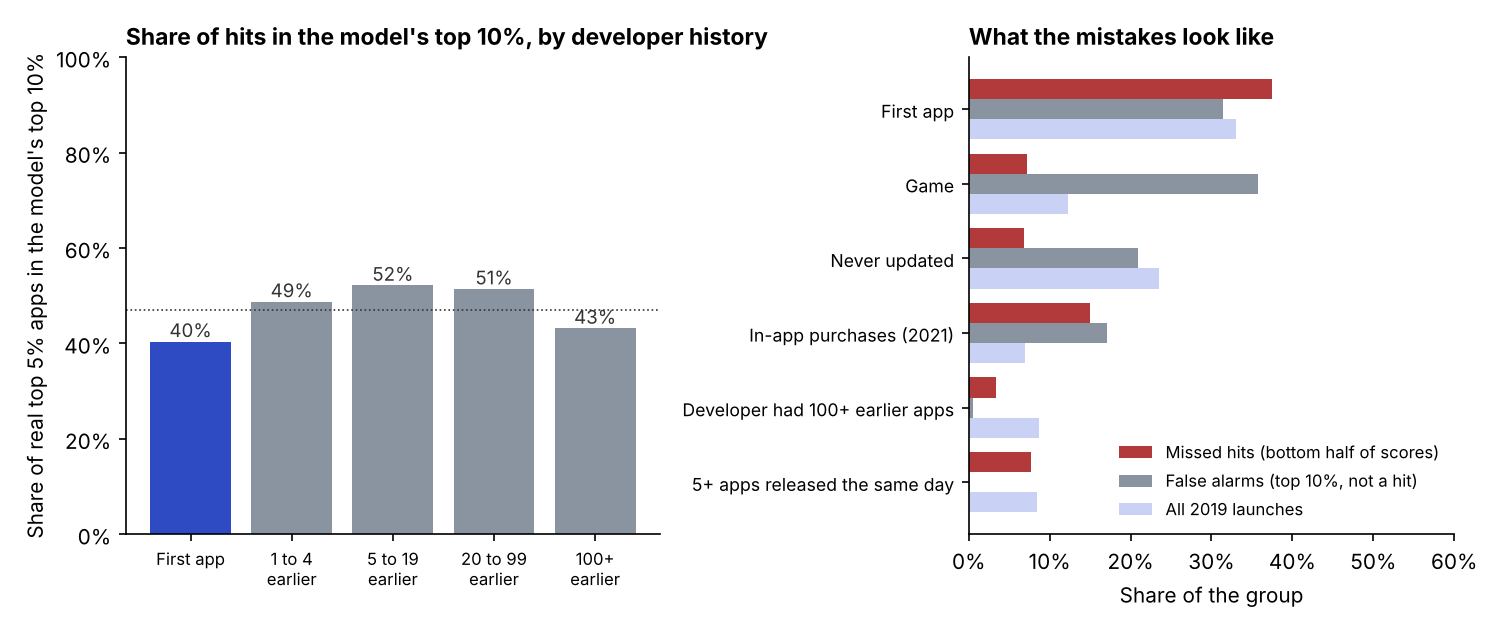
\includegraphics[width=0.98\linewidth]{9_errors.png}
\caption{Error analysis on 2019 launches. Left: share of real hits that land in the model's top 10\%, by developer
history. Right: who the missed hits and false alarms are. 2021-only fields appear here as descriptions, never as
inputs.}
\label{fig:err}
\end{figure}

\paragraph{Errors.} The model's top 10\% contains \RecallOverall{} of all hits, and \PrecisionTop{} of the apps it
flags are hits. Games make up more of the caught hits because their base rate is higher, and ranking within games is a
little worse than within other apps. Figure~\ref{fig:err} shows where it fails.

\section{Time to milestones}

\begin{figure}[!htb]
\centering
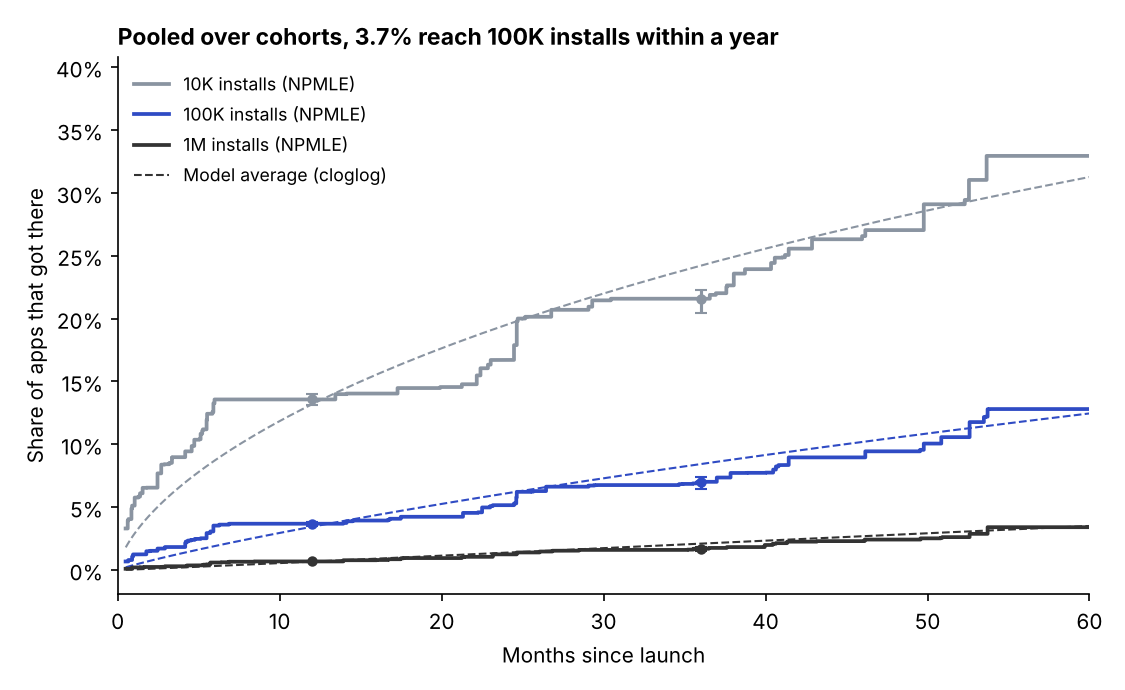
\includegraphics[width=0.62\linewidth]{10_milestone_curves.png}
\caption{NPMLE of the time to 10K, 100K and 1M installs for \WindowApps{} apps launched January 2016 to May 2021,
with cube-root subsampling intervals at 12 and 36 months. Dashed lines are the \Link{} model averaged over apps.}
\label{fig:curves}
\end{figure}

Figure~\ref{fig:curves} shows the pooled NPMLE curves. Within 12 months of launch \FTenKTwelve{}
[\FTenKTwelveLo, \FTenKTwelveHi] of apps reach 10K installs, \FHundredKTwelve{} [\FHundredKTwelveLo,
\FHundredKTwelveHi] reach 100K and \FOneMTwelve{} [\FOneMTwelveLo, \FOneMTwelveHi] reach 1M. At 36 months the
numbers are \FTenKThirtySix{}, \FHundredKThirtySix{} and \FOneMThirtySix{}. These are pooled over launch cohorts,
and they assume every cohort grows at the same pace. The curves are flat between about 6 and 12 months, which is what
the estimator does when newer cohorts did better than older ones at the same age. Raw rates at a single age show the
same thing. Among the \RawApps{} apps 11 to 13 months old (launched mid May to mid July 2020), \RawTenK{} had
reached 10K, \RawHundredK{} had reached 100K and \RawOneM{} had reached 1M, and the 10K share only moves between
\RawFlatLo{} and \RawFlatHi{} across ages 5 to 16 months. The 100K value is below the pooled interval at 12 months.
The subsampling intervals reflect sampling and not cohort drift. In a simulation with a known curve and
\NpmleSimApps{} apps, intervals meant to cover \NpmleSimNominal{} covered \NpmleSimCoverage{}.

Each model is a binary GLM fit to a random sample of \FitSample{} apps. Held-out log loss averaged over both checks and
all milestones was \LLCloglog{} for cloglog, \LLProbit{} for probit and \LLLogit{} for logit, so I treat the three links as a tie and use \Link{}, which was lowest on the folds I scored. In the interleaved check (every fourth launch month held out) the AUC is \IntAUCTenK{}, \IntAUCHundredK{} and
\IntAUCOneM{} for the three milestones and the 100K calibration slope is \IntSlopeHundredK{}. In the forward check
(fit on launches before June 2019, score the two years after) the AUC is \FwdAUCTenK{}, \FwdAUCHundredK{} and
\FwdAUCOneM{}, and \FwdWAUCTenK{}, \FwdWAUCHundredK{}, \FwdWAUCOneM{} within launch month. Log loss beats an age-only
model in every case (forward 100K: \FwdLLHundredK{} vs \FwdAgeLLHundredK{}). The forward check under-predicts. For 100K
the model averages \FwdMeanPredHundredK{} against a real \FwdRateHundredK{}, and near one year of age the calibration
intercepts are \FwdIntYearTenK{}, \FwdIntYearHundredK{} and \FwdIntYearOneM{} with slopes \FwdSlopeYearTenK{},
\FwdSlopeYearHundredK{} and \FwdSlopeYearOneM{} (Figure~\ref{fig:fwd}). Every app in that fit is at least 24 months
old, so the check extrapolates the time curve as well as testing the no-cohort-effect assumption, and with one
snapshot I cannot tell the two apart. I treat the 12-month probabilities as rough. The pooled fit is also off by age. At 5 to 7 months its 10K average is
\RawModelEarly{} against a raw \RawObsEarly{}, and at 17 to 19 months it is \RawModelLate{} against \RawObsLate{}.

\begin{figure}[!htb]
\centering
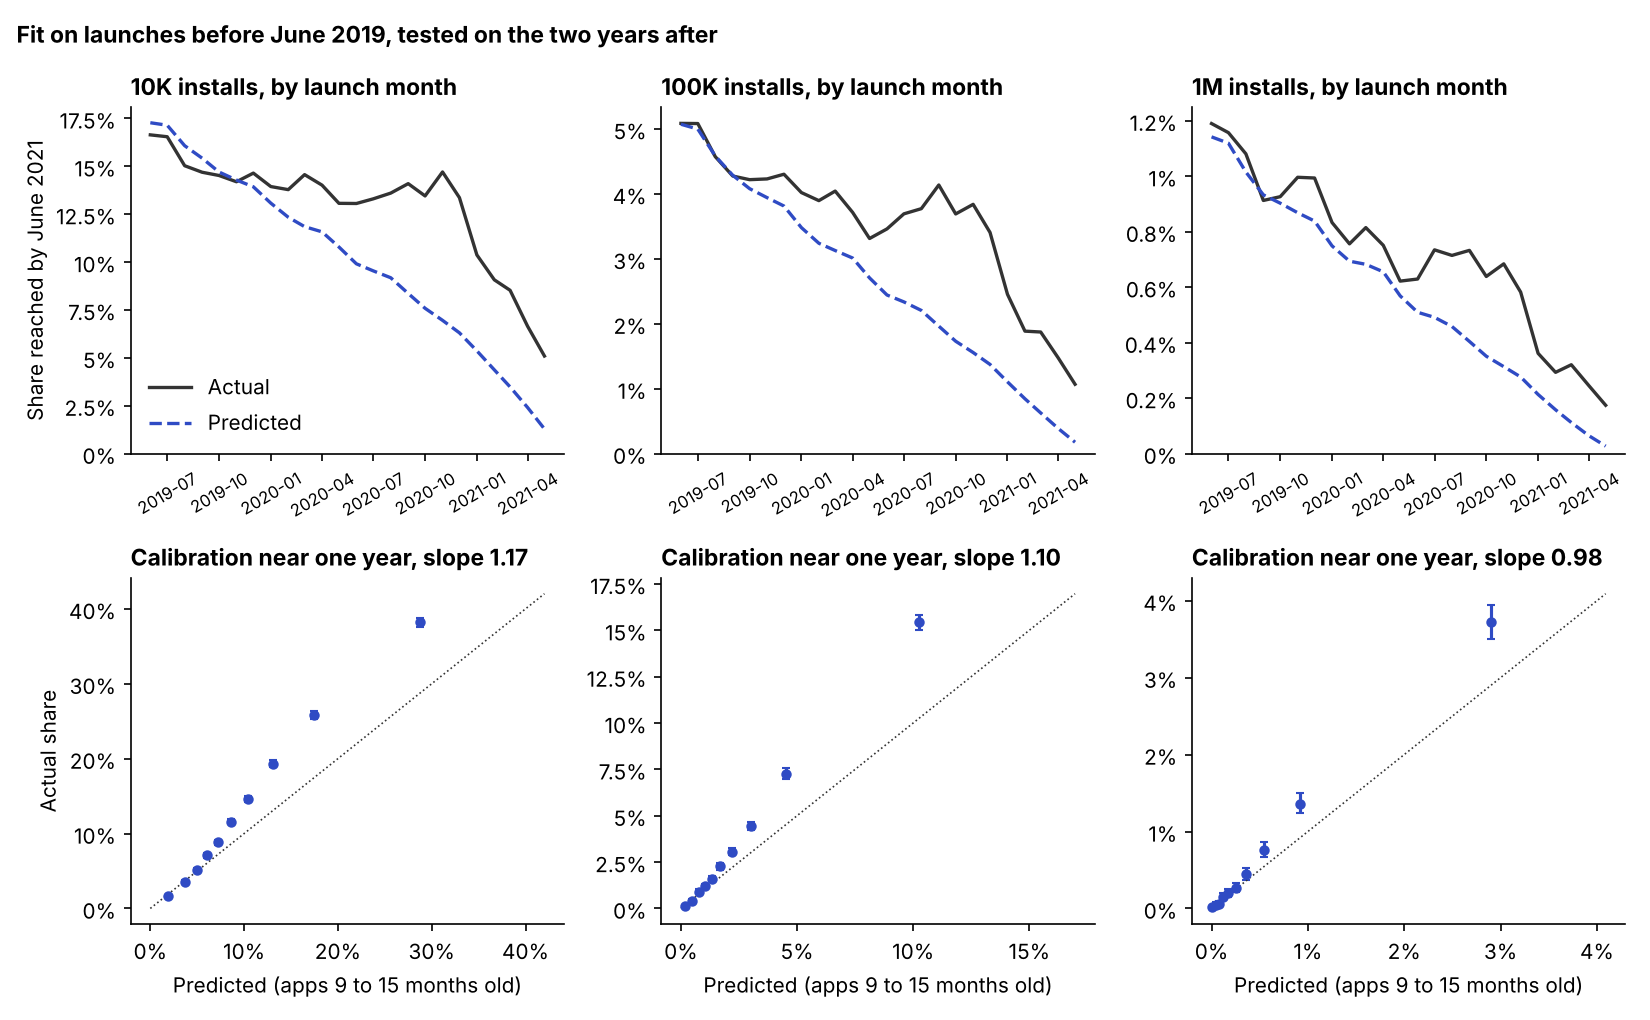
\includegraphics[width=0.84\linewidth]{11_forward_validation.png}
\caption{Forward check. Top: predicted and actual share past each milestone by launch month, for launches the
model never saw. Bottom: reliability for apps 9 to 15 months old.}
\label{fig:fwd}
\end{figure}

\paragraph{Intervals for one app.} The scorer gives two kinds of intervals. The probability interval comes from the
developer-clustered covariance and only reflects parameter uncertainty. The second is a split conformal interval for
where the app will land among apps launched the same month, computed inside 20 bins of the launch score. On random
held-out apps the 50\%, 80\% and 90\% intervals covered \CovFifty{}, \CovEighty{} and \CovNinety{}. Forward in
time, with a score fit before June 2019, the 80\% interval covered \CovEightyFwd{}. It covers less for games
(\CovGames{}). The intervals are wide. On the 0 to 1 scale of launch-month percentiles the mean widths are
\WidthFifty{}, \WidthEighty{} and \WidthNinety{} for the 50\%, 80\% and 90\% intervals (\WidthEightyFwd{} for 80\%
forward), so for one app they only give a rough neighborhood. Coverage by developer history is in
Figure~\ref{fig:cov}.

\begin{figure}[!htb]
\centering
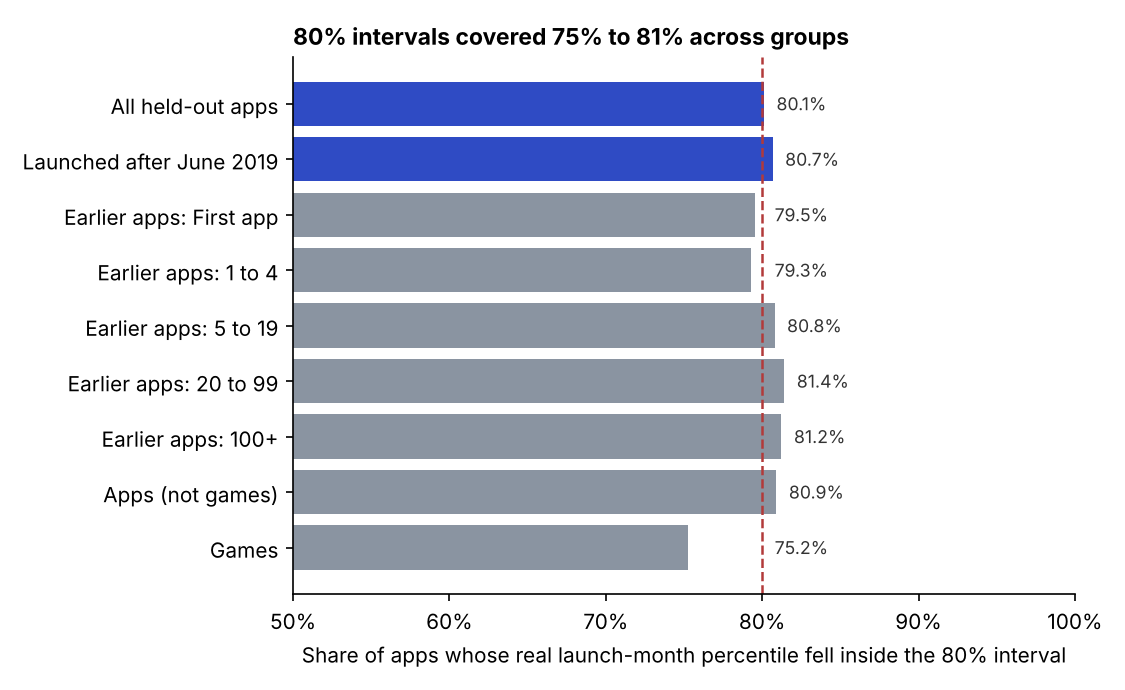
\includegraphics[width=0.5\linewidth]{12_interval_coverage.png}
\caption{Empirical coverage of the 80\% conformal interval.}
\label{fig:cov}
\end{figure}

\section{Categories}

Category carries most of the launch-day signal. A category-only rate scores \AUCBaseCat{}, more than all the developer
and package features together (\AUCStrict{} for the strict model). Averaged over a developer's first apps of 2019 and
2020, the milestone model gives a \SimFirstTenK{} chance of 10K installs within a year in Simulation and \BusFirstTenK{}
in Business. The raw rates for those developers' first apps that were 9 to 15 months old are \SimObsTenK{} in Simulation
(\SimObsApps{} apps, where the model says \SimModelTenK{} at those ages) and \BusObsTenK{} in Business (\BusObsApps{}
apps, model \BusModelTenK{}). Over all developers and the 48 categories, the model's average sat inside the 95\%
interval of the raw rate for \CatInsideTenK{} of categories at 10K and \CatInsideHundredK{} at 100K, and the ratio of
observed to modeled 10K ran from \CatRatioMin{} to \CatRatioMax{}. The model is fine on average and can be off by a
factor of two for one category. Across categories, the share of installs taken by the top 10 apps has a rank
correlation of \TopTenCorr{} with that chance. \texttt{results/study/market.csv} has demand, supply, Gini and HHI for every category.

\section{Monetization: association, not effect}

The old write-up found that apps with both ads and in-app purchases broke out far more often, and the simulator
turned that into a lever. That reading is not supported. The flags were observed in 2021, and an app with users has
every reason to add in-app purchases. Adjusting for category, launch month and developer history, apps with ads and
in-app purchases in 2021 were \RRAdsIapAll{} times as likely as ads-only apps to reach the top 5\% of their launch
month (95\% CI \RRAdsIapAllLo{} to \RRAdsIapAllHi{}). The E-value is \EAdsIapAll{} \citep{vanderweele2017}, which is the risk ratio an
unmeasured factor, or a reverse path from success to monetization, would need with both the flag and the outcome to
explain away the whole association. I cannot rule out a reverse path that strong.

Apps never updated after release are the closest thing to a launch-day listing in this data. Among them the same
ratio is \RRAdsIapNever{} [\RRAdsIapNeverLo, \RRAdsIapNeverHi], and among updated apps it is \RRAdsIapUpd{}
[\RRAdsIapUpdLo, \RRAdsIapUpdHi]. Hits were never updated \NeverHits{} of the time against \NeverRest{} for the rest,
so this split is itself selected on something downstream of success. Among hits, \IapHitsUpd{} of updated apps had
in-app purchases against \IapHitsNever{} of never-updated apps, a ratio of about \IapHitsRatio{}, which is below the \EAdsIapAll{}
that a reverse path would need. I read the split as a hint about timing and nothing stronger. None of these numbers is the effect of choosing a
business model, and the next version of the simulator should not present them as levers.

\section{Limitations}
\label{sec:limits}

\begin{itemize}
\item Survivorship. Only apps listed in June 2021 are observed. Older cohorts have lost more failures, which biases
the long-horizon parts of the milestone curves upward and makes developer history run low.
\item One snapshot. Training labels for the 2018 cohort were also measured in 2021, so a true backtest is not possible
and the temporal split is the closest I can get. The milestone model's no-cohort-effect assumption can only be checked out of sample, and the forward
check under-predicts. The pooled curves and their intervals ignore cohort drift.
\item Category and title are 2021 values. I treat them as launch information because developers pick them before
launch, but either can be edited. The strict model without them scores \AUCStrict{}, and dropping the title features alone
lowers the ablation AUC from \AblLaunch{} to \AblNoTitle{}.
\item The probability intervals are parameter intervals. They don't cover model error. The conformal intervals do
have checked coverage, but only for the launch-month percentile, and they cover less for games.
\item The data covers Google Play only, and nothing after June 2021.
\end{itemize}

\section{Reproducibility}

Everything runs from \texttt{make all} after \texttt{bash get\_data.sh}. Every number in this paper is written to
\texttt{numbers.tex} by \texttt{paper/make\_numbers.py} from the saved results. Tests (\texttt{make test}) run the full
pipeline on a small synthetic dataset, check the metric code against scikit-learn, check the survival estimators on
data with a known answer, and check that the exported model reproduces the fitted model to $10^{-9}$ in Python and
JavaScript.

\bibliographystyle{plainnat}
\begin{thebibliography}{9}
\bibitem[Groeneboom and Wellner(1992)]{groeneboom1992}
P.~Groeneboom and J.~A. Wellner. \emph{Information Bounds and Nonparametric Maximum Likelihood Estimation}.
Birkh\"auser, 1992.
\bibitem[Politis and Romano(1994)]{politis1994}
D.~N. Politis and J.~P. Romano. Large sample confidence regions based on subsamples under minimal assumptions.
\emph{Annals of Statistics}, 22(4), pages 2031 to 2050, 1994.
\bibitem[Prakash(2021)]{prakash2021}
G.~Prakash. Google Play Store dataset (2.3M+ apps). GitHub, 2021.
\bibitem[Sen et~al.(2010)]{sen2010}
B.~Sen, M.~Banerjee and M.~Woodroofe. Inconsistency of bootstrap: the Grenander estimator. \emph{Annals of
Statistics}, 38(4), pages 1953 to 1977, 2010.
\bibitem[VanderWeele and Ding(2017)]{vanderweele2017}
T.~J. VanderWeele and P.~Ding. Sensitivity analysis in observational research: introducing the E-value.
\emph{Annals of Internal Medicine}, 167(4), pages 268 to 274, 2017.
\end{thebibliography}

\end{document}
